\documentclass[a4paper]{article}
\usepackage[utf8]{inputenc}
\usepackage[spanish, es-tabla, es-noshorthands]{babel}
\usepackage[table,xcdraw]{xcolor}
\usepackage[a4paper, footnotesep = 1cm, width=22cm, top=2.5cm, height=25cm, textwidth=20cm, textheight=25cm]{geometry}
%\geometry{showframe}

\usepackage{tikz}
\usepackage{amsmath}
\usepackage{amsfonts}
\usepackage{amssymb}
\usepackage{float}
\usepackage{graphicx}
\usepackage{caption}
\usepackage{subcaption}
\usepackage{multicol}
\usepackage{multirow}
\usepackage{wrapfig}
\setlength{\doublerulesep}{\arrayrulewidth}
\usepackage{booktabs}

\usepackage{hyperref}
\hypersetup{
    colorlinks=true,
    linkcolor=blue,
    filecolor=magenta,      
    urlcolor=blue,
    citecolor=blue,    
}

\newcommand{\note}[1]{
	\begin{center}
		\huge{ \textcolor{red}{#1} }
	\end{center}
}

\setcounter{topnumber}{2}
\setcounter{bottomnumber}{2}
\setcounter{totalnumber}{4}
\renewcommand{\topfraction}{0.85}
\renewcommand{\bottomfraction}{0.85}
\renewcommand{\textfraction}{0.15}
\renewcommand{\floatpagefraction}{0.8}
\renewcommand{\textfraction}{0.1}
\setlength{\floatsep}{5pt plus 2pt minus 2pt}
\setlength{\textfloatsep}{5pt plus 2pt minus 2pt}
\setlength{\intextsep}{5pt plus 2pt minus 2pt}

\newcommand{\quotes}[1]{``#1''}
\usepackage{array}
\newcolumntype{C}[1]{>{\centering\let\newline\\\arraybackslash\hspace{0pt}}m{#1}}
\usepackage[american]{circuitikz}
\usetikzlibrary{calc}
\usepackage{fancyhdr}
\usepackage{units} 

\graphicspath{{../Ejercicio-1/}{../Ejercicio-2/}{../Ejercicio-3/}{../Ejercicio-4/}{../ParteI/}{../ParteII/}{../ParteIII/}{../ParteIV/}}

\pagestyle{fancy}
\fancyhf{}
\lhead{22.14 - Electrónica IV}
\rhead{Mechoulam, Lambertucci, Londero}
\rfoot{Página \thepage}


\begin{document}

\subsection{Introducción}

Para el estudio del modo discontinuo de la fuente estudiada anteriormente, se calculó la corriente media $I_{L_b} = I_{o_b}$ de boundary de la bobina, la cual es la misma que la corriente media de salida. El valor anterior de $\Delta I_L$ fue de $494.404mA$ por lo que la corriente media de boundary será

\begin{equation}
I_{L_b} = \frac{\Delta I_L}{2} = 247.202mA
\label{ej4:eq:il_boundary}
\end{equation}

Por esta razón, si la corriente de salida es menor que $I_{L_b}$, la fuente trabajará en modo discontinuo. Se seleccionó una resistencia de salida de $R_o = 500\Omega > R_{o_{min}} = \frac{V_o}{I_{L_b}} = 97.1\Omega$ para obtener resultados más significantes y se utilizó un duty cycle $D = 0.665$ para conservar los $24V$ de salida requeridos. A continuación se detallan las curvas simuladas.

\begin{figure}[H]
	\centering
	\begin{minipage}{0.495\textwidth}
		\centering
		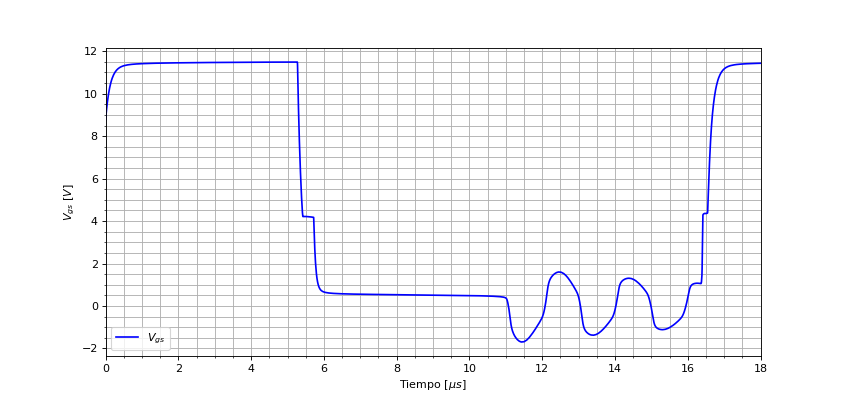
\includegraphics[width=\textwidth]{ImagenesEjercicio-4/vgs} % first figure itself
		\caption{Tensión $V_{gs}$ en modo discontinuo.}
		\label{ej4:fig:vgs}
	\end{minipage}\hfill
	\begin{minipage}{0.495\textwidth}
		\centering
		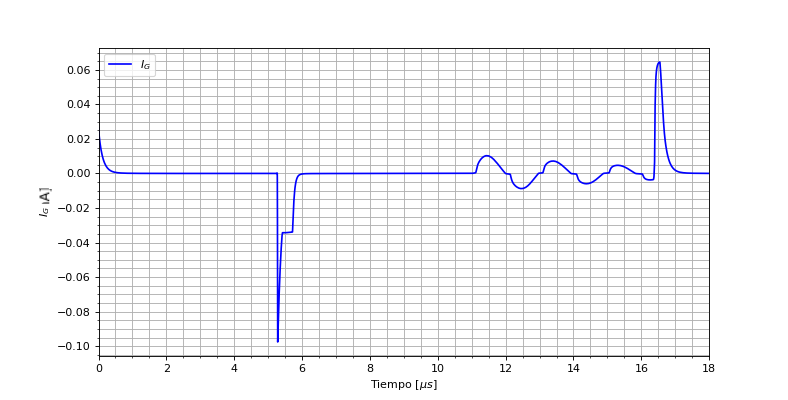
\includegraphics[width=\textwidth]{ImagenesEjercicio-4/ig} % second figure itself
		\caption{Corriente $I_{g}$ en modo discontinuo.}
		\label{ej4:fig:ig}
	\end{minipage}
\end{figure}

\begin{figure}[H]
	\centering
	\begin{minipage}{0.495\textwidth}
		\centering
		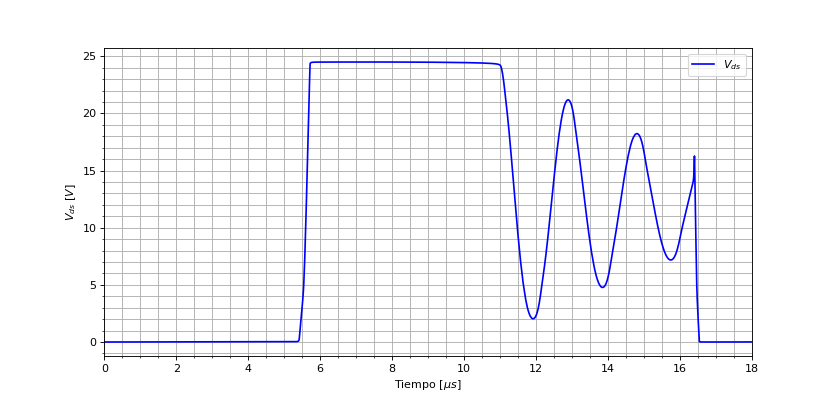
\includegraphics[width=\textwidth]{ImagenesEjercicio-4/vds} % first figure itself
		\caption{Tensión $V_{ds}$ en modo discontinuo.}
		\label{ej4:fig:vds}
	\end{minipage}\hfill
	\begin{minipage}{0.495\textwidth}
		\centering
		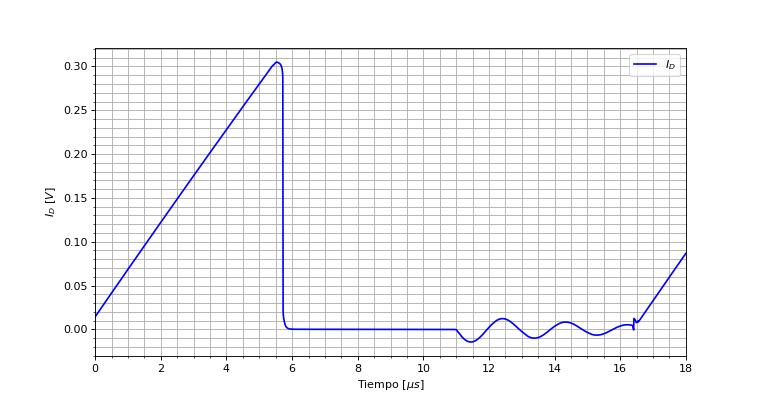
\includegraphics[width=\textwidth]{ImagenesEjercicio-4/id} % second figure itself
		\caption{Corriente $I_{D}$ en modo discontinuo.}
		\label{ej4:fig:id}
	\end{minipage}
\end{figure} 

\begin{figure}[H]
	\centering
	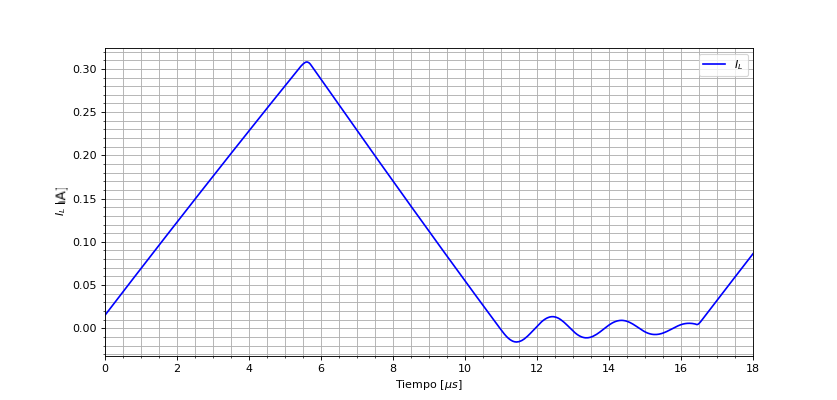
\includegraphics[width=0.7\linewidth, page=1]{ImagenesEjercicio-4/il}
	\caption{Corriente de la bobina en modo discontinuo.}
	\label{ej4:fig:il}
\end{figure}

Se 

\end{document}